% !TEX root =  ../main.tex

\begin{figure*}[t]

    \centering
%    \begin{subfigure}[b]{0.3\textwidth}
%        \centering
%        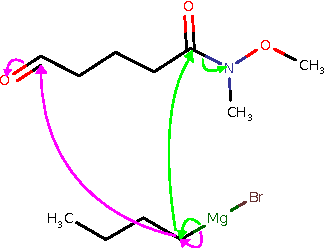
\includegraphics[height=1.2in]{imgs/textbook/reactants2}
%        %\caption{}
%    \end{subfigure}%
    \begin{subfigure}[b]{0.35\textwidth}
        \centering
        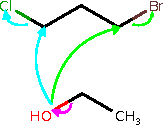
\includegraphics[height=0.9in]{imgs/textbook/reaction3}\\\vspace{0.1in}
        %\caption{}
    \end{subfigure}%
    \hfill
     \begin{subfigure}[b]{0.6\textwidth}
        \centering
        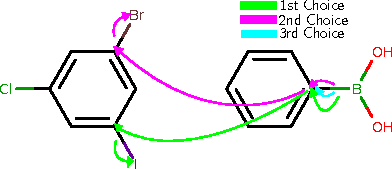
\includegraphics[height=1.1in]{imgs/textbook/reaction7}
        %\caption{}
    \end{subfigure}
%    \vspace{-1em}
	\caption{In (left) 2nd-order nucleophilic substitutions $S_N 2$-reactions, and (right) Suzuki-couplings, halides lower in the period table usually react preferably ($I>Br>Cl$). In both cases, our model has correctly picked up this trend.}
	\label{fig:qualitative}
\end{figure*}



\subsection{Qualitative Analysis}

Complex molecules often feature several potentially reactive functional groups $r=\{F_1,...,F_N\}$, which compete for reaction partners. 
To predict the selectivity, that is which functional group will predominantly react in the presence of other groups, 
students of chemists learn heuristics and trends, 
which have been established over the course of three centuries of experimental observation.
To qualitatively study whether the model has learned such trends from data we queried the model with several typical text book examples from the chemical curriculum (see Figure \ref{fig:qualitative} and appendix). 
We found that the model predicts most examples correctly. In the few incorrect cases, interpreting the model's output reveals that the model made chemically plausible predictions.

